%\documentclass{book}
\documentclass{article}                            %for shorter notes
\usepackage{graphicx}                              %for PNG images (pdflatex)
%\usepackage{graphics}                              %for EPS images (latex)
\usepackage[linkbordercolor={1.0 1.0 0.0}]{hyperref} %for \url tag
\usepackage{color}                                 %for defining custom colors
\usepackage{framed}                                %for shaded and framed paragraphs
\usepackage{textcomp}                              %for various symbols, e.g. Registered Mark
\usepackage{geometry}                              %for defining page size
\usepackage{longtable}                             %for breaking tables
%
\geometry{verbose,a4paper,tmargin=2.5cm,bmargin=2.5cm,lmargin=2.5cm,rmargin=2cm}
\hypersetup{
  pdfauthor = {Ivan Marton},
  pdftitle = {ISIS Technical handbook},
  pdfsubject = {ISIS Technical handbook},
  pdfkeywords = {Paper,keyword,comma-separated},
  pdfcreator = {PDFLaTeX with hyperref package},
  pdfproducer = {PDFLaTeX}
}
%
\bibliographystyle{IEEEtran}                       %a nice bibliography style
%
\def\efill{\hfill\nopagebreak}%
\hyphenation{Nordu-Grid}
\setlength{\parindent}{0cm}
\setlength{\FrameRule}{1pt}
\setlength{\FrameSep}{8pt}
\addtolength{\parskip}{5pt}
\renewcommand{\thefootnote}{\fnsymbol{footnote}}
\renewcommand{\arraystretch}{1.3}
\newcommand{\dothis}{\colorbox{shadecolor}}
\newcommand{\globus}{Globus Toolkit\textsuperscript{\textregistered}~2~}
\newcommand{\GT}{Globus Toolkit\textsuperscript{\textregistered}}
\newcommand{\ngdl}{\url{http://download.nordugrid.org/}~}
\definecolor{shadecolor}{rgb}{1,1,0.6}
\definecolor{salmon}{rgb}{1,0.9,1}
\definecolor{bordeaux}{rgb}{0.75,0.,0.}
\definecolor{cyan}{rgb}{0,1,1}
%
%----- DON'T CHANGE HEADER MATTER
\begin{document}
\def\today{\number\day/\number\month/\number\year}

\begin{titlepage}

\begin{tabular}{rl}
\resizebox*{3cm}{!}{
\includegraphics{logo-knowarc.png}}
\end{tabular}

\hrulefill

%-------- Change this to Knowarc_D<w>.<d>-<n>_<yy>

%{\raggedleft Knowarc\_D0.0-0\_00\par}

{\raggedleft \today\par}

\vspace*{2cm}

%%%%---- The title ----
{\centering \textsc{\Large ISIS Information Indexing Service}\Large \par}
\vspace*{0.5cm}
    
%%%%---- A subtitle, if necessary ----
{\centering \textit{\large Technical handbook}\large \par}
    
\vspace*{1.5cm}
%%%%---- A list of authors ----
{\centering \large Ivan Marton\footnote{martoni@niif.hu} \large \par}
    
%%%%---- An abstract - if style is article ----
%\begin{abstract}
%The abstract
%\end{abstract}
\end{titlepage}
\tableofcontents                          %Comment if use article style
\newpage
%\chapter{Preface}
\section{Introduction}
\label{Introduction}

\section{Components}
\label{Components}
\subsection{Registrant}
\label{Registrant}
The Registrant is active module of the HED (Hosting Environment Daemon) which is bound to a set of ISIS's. In practice, the configuration part of the Registrant contains exactly one ISIS to bind, and the Registrant will collect the necessary information about the other ISIS's belonging to the same network.\par
If the administrator wants to use more then one network for registering his services then more then one Registrant have to be instanced for this purpose. In this case, the default Registrant will be used for registering every services that isn't configured in a different way. \par
The registration can be done once or periodically. It based on the configuration of the Registrant as default behavior but can be overwritten for every service separately.\par
The Registrant is doing the message aggregation of every service belongs to it if it's possible. The algorithm of the Registrant is following:
\begin{framed}
  Registrant - pseudo algorithm\\
  \\
  \verb#// Initialize phase#\\
  \verb#Read the configuration and store the information about the services in a list#\\
  \verb#do { // Cyclic phase in a different Thread#\\
  \verb# wake_up_time = now();#\\
  \verb# messages = null;#\\
  \verb#  if ( 0 < count(service where service.next_run <= wake_up_time)) {#\\
  \verb#    foreach( service where service.next_run <= wake_up_time) {#\\
  \verb#      messages.add(service.RegistrationCollector);#\\
  \verb#      service.next_run = wake_up_time + service.period;#\\
  \verb#    }#\\
  \verb#    if (0 < count(messages)) {#\\
  \verb#      sent_message = assemble message with headers(messages);#\\
  \verb#      send(sent_message);#\\
  \verb#    }#\\
  \verb#  } else {#\\
  \verb#    sleep(min(service.next_run) - now()); #\\
  \verb#  }#\\
  \verb#} while(true)#\\
\end{framed}
There is a minimum value of the period defined. If the settings is less then 2 minutes then it will be replaced with this value.
Before sending the information received from the services (\textbf{Service Advertisement}, see Section \ref{Service Advertisement}), the Registrant extend them some additional data (\textbf{Service Advertisement Metadata}). This part of the message contains the following information:
\begin{itemize}
  \item GenTime: (Generation Time) The actual timestamp (called wake\_up\_time in the pseudo code)
  \item Expiration: (The time of Service Advertisement's expiration.)  Generation Time + Renewal period length.
  \item Source: The Endpoint of the Service
  \item Status: Status of the Service Advertisement.
\end{itemize}
A \textbf{Registration Entry} contains a \textbf{Service Advertisement} and a corresponding \textbf{Service Advertisement Metadata}.\par
The \textbf{Registration Message} is the one that will be sent to an ISIS service. This message is consists of more \textbf{Registration Entry} and at most \textbf{Registration Header}.  This embedded structure can be shown on Figure \ref{fig:RegistrationMessage}.
\begin{figure}[ht]
\centering{{\scalebox{0.6}{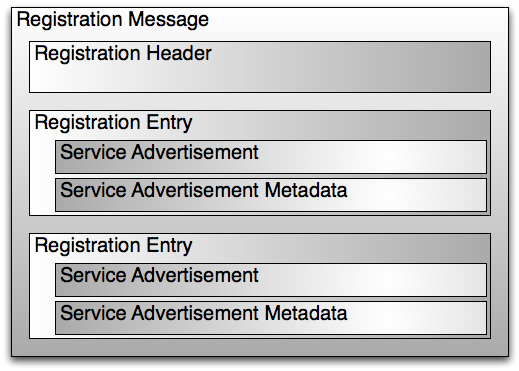
\includegraphics{RegistrationMessage.png}}}
\caption{\label{fig:RegistrationMessage}Embedded structure of Registration Message} }
\end{figure}
\subsection{Services}
\label{Services}
The service developers have to ensure that the services are able to provide the necessary information about themselves. It can be easily done by implementing the proper interface of the Arc::Service class. It means to fill the RegistrationCollector function with the necessary code parts to assemble the always up-to-date status information about the service and anything else wants to be advertised. This information package is called \textbf{Service Advertisement}.\par
\label{Service Advertisement}
The \textbf{Service Advertisement} can contains any information wants to advertised but the mandatory elements are the following attributes these one have to be present:
\begin{itemize}
  \item Service ID: A globally unique identifier.
  \item Service Type: The Glue2 type of service.
  \item Endpoint URL: The URL where the service can be achieved.
\end{itemize}
\subsection{ISIS Service}
\label{ISIS Service}
The ISISs perform two completely different function. On the one hand they are working as ordinary HED services, and on the other hand maintain a peer-to-peer network between each other.
\subsubsection{Service functions}
\label{ISIS Service functions}
Every ISIS service has two different interfaces:
\begin{itemize}
  \item WSRF interface
  \item service specific interface
\end{itemize}
The WSRF interface returns the service specific information expect of the stored database. (The Property Document doesn't contains the Activities that are the Registration Entries in this case.) The service specific interface is for retrieve these data. This interface has 5 operation defined:
\begin{itemize}
  \item Register\par
  The register operation is accessed by the Registrant. See Section \ref{Registration} for further details.
  \item RemoveRegistration\par
  This operation is used for requesting the removal of a list of zero or more Registration Entries stored in the Information System. The attribute of this operation is a list of Service IDs. Every entry belonging to any of the given Service ID will be removed.
  \item GetRegistrationStatuses\par
  This operation is used for requesting the current status(es) of zero or more Registration Entries previously pushed into the system by the Register operation. The operation receives a list of Service ID as its input and returns a list of <ServiceID, Status> pairs.
  \item GetISISList\par
  The operation is used for obtaining a list of known ISIS instances from any particular ISIS. Clients can then use the obtained list to run direct queries against the ISIS instances.  The operation is provided for fault tolerance and for providing optional performance boost. This operation returns the known peer-to-peer neighbors. If you are interested in every known ISIS then they can be queried with the Query operation because they are ordinary services registered into the Information System.
  \item Query
  The operation is used for request any kind of queries related to the Indexing Database. For providing as much flexibility as possible any XQuery searches can be executed. This operation is accessed by clients. For an example and further details see Section \ref{Query data}. 
\end{itemize}

\subsubsection{Peer-to-Peer functions}
\label{ISIS Peer-to-Peer functions}
\subsection{Client}
\label{Client}
The client part of the information service is for querying the data stored in the database of the ISIS services. This is implemented as a part of the ARCLib and using the ISIS service's interface for the various data queries. For further details see Section \ref{Query data}.  
\section{Operations}
\label{Operations}
The different operations are performed by different Information system components. These cases are described below in the dedicated subsections. 
\subsection{Registration}
\label{Registration}
The registration operation is done by the Registrants and described in Section \ref{Registrant}. An example layout can be shown on Figure \ref{fig:RegistrationMessage}. In this configuration there is two different Registrant configured in one HED for three services. Let the \textit{Registrant A} the default Registrant and the services configured in the following way:\par
\begin{itemize}
  \item Service 1: There is no Registrant configured so the default one will register it.
  \item Service 2: The \textit{Registrant A} is configured explicitly.
  \item Service 3: The \textit{Registrant B} is configured explicitly.
\end{itemize}
In the sketched case the Service 1 and 2 are handled equivalently by \textit{Registrant A} and Service 3 by \textit{Registrant B}.\par
In the first step the information collection from the first handled services is done parallel (\textit{A1}-\textit{A2}, \textit{B1}-\textit{B2}). The retrieved data are stored and other services are queried if there is any (\textit{A3}, \textit{A4}). Finally, the aggregated information is sent to the corresponding ISISs independently from each other (\textit{A5}, \textit{B5}).\par
\begin{figure}[ht]
\centering{{\scalebox{0.6}{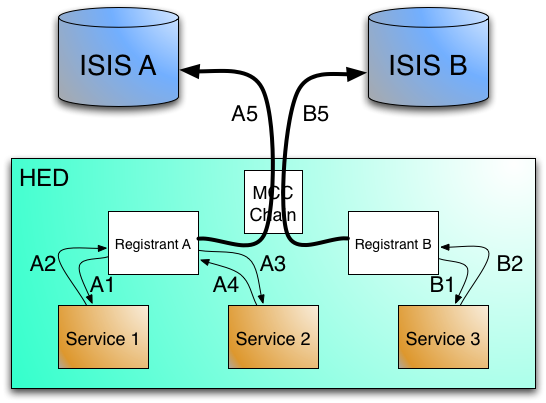
\includegraphics{Registration.png}}}
\caption{\label{fig:RegistrationMessage}Overview of the registration operation} }
\end{figure}
This registration operation is done once during the start-up phase and cyclic later by right of the (per service) configured periods. This periodical operation follows the algorithm described in Section \ref{Registrant}, and do every possible message aggregation.
\subsection{Query data}
\label{Query data}

\subsection{Configuration}
\label{Configuration}
The configuration of the different modules can be done through the ARC Configuration file. The format of these entries is shown by the relevant XSD Schema files.

\begin{framed}
Registrant.xsd\\
\\
\verb#<?xml version="1.0" encoding="UTF-8"?>#\\
\verb#<xsd:schema#\\
\verb#  xmlns:xsd="http://www.w3.org/2001/XMLSchema"#\\
\verb#  xmlns:registrant="http://www.nordugrid.org/schemas/RegistrantConfig/2008"#\\
\verb#  xmlns:arcConfig="http://www.nordugrid.org/schemas/ArcConfig/2007"#\\
\verb#  targetNamespace="http://www.nordugrid.org/schemas/RegistrantConfig/2008"#\\
\verb#  elementFormDefault="qualified">#\\
\verb# #\\
\verb#    <xsd:complexType name="Registrant_Type">#\\
\verb#        <!-- This element defines configuration of Information #\\
\verb#            Registration interface. -->#\\
\verb#        <xsd:sequence>#\\
\verb#            <!-- Period specifies how often registration to be done in seconds.#\\
\verb#                The missing or 0 value means a non period registration. -->#\\
\verb#            <xsd:element name="Period" type="xsd:nonNegativeInteger"/>#\\
\verb#            <!-- URL specifies contact endpoint of a bootstrap Information#\\
\verb#                Registration service. Further ISIS's adresses will be queried#\\
\verb#                from this service. -->#\\
\verb#            <xsd:element name="ISIS_URL" type="xsd:string" />#\\
\verb#            <!-- Optional KeyPath, CertificatePath, ProxyPath and CACertificatesDir#\\
\verb#                are paths to files storing X509 credentials used for establishing#\\
\verb#                connections. -->#\\
\verb#            <xsd:element name="KeyPath" type="xsd:string" minOccurs="0" />#\\
\verb#            <xsd:element name="CertificatePath" type="xsd:string" minOccurs="0" />#\\
\verb#            <xsd:element name="ProxyPath" type="xsd:string" minOccurs="0" />#\\
\verb#            <xsd:element name="CACertificatesDir" type="xsd:string" minOccurs="0" />#\\
\verb#        </xsd:sequence>#\\
\verb#    </xsd:complexType>#\\
\verb#    <xsd:element name="Registrant" type="registrant:Registrant_Type"/>#\\
\verb# #\\
\verb#    <!-- Optional element for Service element overriding the default Period length. -->#\\
\verb#    <xsd:element name="Period" type="xsd:nonNegativeInteger"/>#\\
\verb# #\\
\verb#</xsd:schema>#\\
\end{framed}

%Advanced Resource Connector (ARC) was invented by
%NorduGrid~\cite{nordugrid}. This \textit{middleware}\index{middleware}
%uses \GT~4 by Globus.

%In expressions, the following operands are allowed:
%\begin{shaded}
%  \verb#=   !=   >   <   >=   <=#
%\end{shaded}

%\begin{framed}
%  Examples of URLs are:\\
%  \\
%  \verb#http://grid.domain.org/dir/script.sh#\\
%  \verb#gsiftp://grid.domain.org:2811;threads=10/dir/input_12378.dat#\\
%  \verb#ldap://grid.domain.org:389/lc=collection1,rc=Nordugrid,dc=nordugrid,dc=org#\\
%  \verb#rc://grid.domain.org/lc=collection1,rc=Nordugrid,dc=nordugrid,dc=org/zebra/f1.zebra#
%  \verb#file:///home/auser/griddir/steer.cra#\\
%\end{framed}

%\subsection{Subsection}
%\label{sec:subsection}

%\begin{figure}[ht]
%\centering{{\scalebox{0.9}{
\includegraphics{logo-knowarc.png}}}
%\caption{\label{fig:myfigure1}The figure shows a logo.} }
%\end{figure}


\bibliography{grid}
\end{document}
